
\documentclass[12pt,epsfig,color,russian]{article}
\usepackage[russian]{babel}
\usepackage{epsfig}
\usepackage{color}

\topmargin=0cm
\hoffset -30mm
\voffset -12mm
\setlength{\unitlength}{1mm}
\parindent=10mm
\textheight=250mm
\textwidth=185mm
\pagestyle{empty}

\begin{document}
\sf\Large


\centerline{\underline{\Huge\bf ДИНАМИКА}}

\centerline{\sl изучает взаимодействие тел, приводящее к изменению их движения}
\vspace{2mm}
\underline{\bf Первый закон Ньютона (принцип инерции)}
\begin{center}
\fbox{\parbox{180mm}{\color{blue}\bf Всякое тело сохраняет состояние покоя или равномерного и прямолинейного движения, пока
воздействие со стороны других тел не заставит его изменить это состояние.}}\\[1mm]
(Здесь тело -- как материальная точка, то есть, вращение исключается.)
\end{center}

Наблюдения: 1зН справедлив не для каждой системы отсчета.

\fbox{Инерциальная система} -- та, по отношению к которой 1зН выполняется.

Гелиоцентрическая система. Всякая система, движущаяся относительно нее равномерно и прямолинейно.
\fbox{\color{blue}Инерциальные системы существуют.}\\

\underline{\bf Второй закон Ньютона}
\begin{center}
\fbox{\parbox{180mm}{\color{blue}\bf Изменение движения пропорционально приложенной силе и происходит в том направлении, в каком действует сила.}}\\[1mm]
\end{center}
Физ. величина СИЛА характеризует воздействие одних тел на другие, в результате которого тела приобретают ускорение.
\begin{displaymath}
 f=k\cdot a\;\;\;\;\;\;\;\;\vec{f}=k\cdot\vec{a}
 \end{displaymath}
Более удобное измерение силы: пружинный динамометр\\
 \setlength{\unitlength}{1mm}
  \begin{picture}(180,40)(0,0)
   %\put(0,0){\framebox(180,40)[b]{}}
   \put(15,0){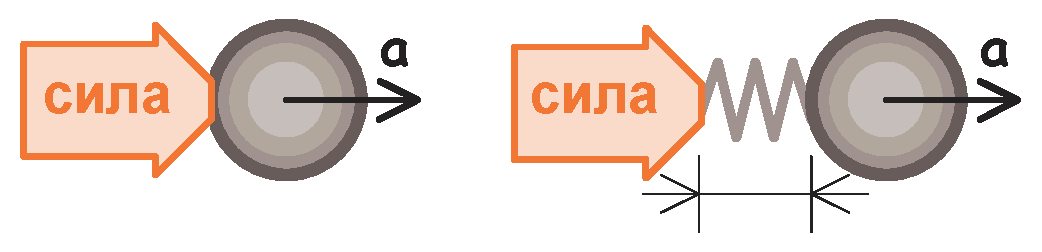
\includegraphics{GP003F01.eps}}
  \end{picture}\\[1mm]
Опыт: {\bf разные} тела от {\bf одинаковой} силы получают {\bf разные} ускорения. Это свойство тел -- физ. величина ИНЕРЦИОННАЯ МАССА.\\
Ньютон: МАССА - это мера количества материи в теле {\sl (не совсем верно)}. МАССА - это именно мера инерции.\\
М.В.Ломоносов: масса изолированной системы = const.
\begin{displaymath}
 \vec{a}=k\cdot\vec{f}/m
 \end{displaymath}
\newpage
Упругие силы, силы тяготения. \underline{\bf Силы трения} -- молекулярное взаимо\-действие между соприкасающимися телами. Трение внешнее (между телом и другими телами; трение покоя) и внутреннее (движение жидкостей и газов).

Сила трения всегда направлена противоположно скорости. Чтобы тело двигалось без ускорения, надо, чтобы внешняя сила уравновешивала силу трения.

 \setlength{\unitlength}{1mm}
  \begin{picture}(180,35)(0,0)
   %\put(0,0){\framebox(180,40)[b]{}}
   \put(10,0){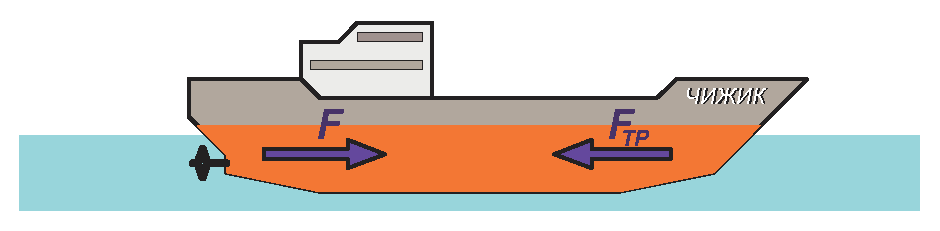
\includegraphics{GP003F02.eps}}
  \end{picture}\\[1mm]

Парашютист: 60 м/с (открытие парашюта) => 5-6 м/с.

Сила трения скольжения приблизительно пропорциональна сжи\-мающей силе $F_n$:
\begin{displaymath}
 F_{TP}\simeq\chi\cdot F_n
 \end{displaymath}

 \setlength{\unitlength}{1mm}
  \begin{picture}(180,55)(0,0)
   %\put(0,0){\framebox(180,40)[b]{}}
   \put(45,0){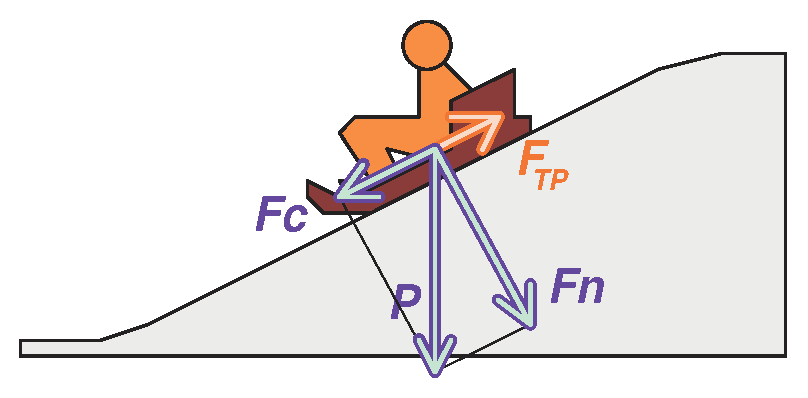
\includegraphics{GP003F03.eps}}
   \put(0,50){\makebox(0,0)[tl]{\parbox{60mm}{коэффициент трения $\chi$ зависит от состояния поверхностей и от скорости скольжения}}}
  \end{picture}\\[1mm]

 \setlength{\unitlength}{1mm}
  \begin{picture}(180,55)(0,0)
   %\put(0,0){\framebox(180,40)[b]{}}
   \put(5,0){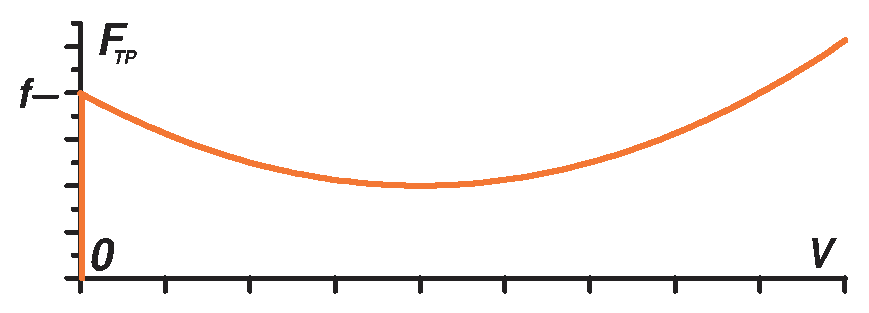
\includegraphics{GP003F04.eps}}
   \put(80,40){\makebox(0,0)[c]{\parbox{85mm}{При V=0 сила трения может быть от 0 до некоего максимума $f$, а при начале движения снижается}}}
   \put(178,30){\makebox(0,0)[tr]{\bf авто: ABS}}
  \end{picture}
\newpage
Рассмотрим движение под действием постоянной силы $\vec{f}$ за время $\Delta t$. Используя 2зН, получим:
\begin{displaymath}
  k\cdot\frac{\vec{f}}{m}=\vec{a}=\frac{\vec{v_2}-\vec{v_1}}{\Delta t}
\end{displaymath}
или, домножив на $m$ и $\Delta t$ :
\begin{displaymath}
 m\vec{v_2}-m\vec{v_1} = k\cdot\vec{f}  \Delta t
\end{displaymath}
Величина $m\vec{v}$ имеет большой физический смысл и называется КОЛИЧЕСТ\-ВО ДВИЖЕНИЯ или ИМПУЛЬС (обозначается как $\vec{p}$ -- от англ. {\sl pulse}).
\begin{displaymath}
\vec{p}\equiv m\vec{v}\hspace{40mm} \frac{\vec{dp}}{dt} = k\cdot\vec{f}
\end{displaymath}

Еще одно определение СИЛЫ: Сила -- векторная величина, пропорцио\-нальная вызываемому ею изменению импульса в единицу времени.

Величина $\vec{f}\Delta t$ тоже имеет персональное название -- ИМПУЛЬС СИЛЫ.

Если положить коэф-т $k$ равным 1, то можно установить единицы измерения для $f$.
\begin{itemize}
\item CGS: $[m]$= г, $\;\;[a]$= см/с$^2\;\;\;\;\Rightarrow\;\;\;[f]$= дина = г$\cdot$см/с$^2$
\item SI: $\;\;\;[m]$= кг, $\;[a]$= м/с$^2\;\;\;\;\Rightarrow\;\;\;[f]$= Ньютон = кг$\cdot$м/с$^2 = 10^5$дин
\end{itemize}
\vspace{2mm}

\underline{\bf Механический принцип относительности (Галилей)}

1зН -- частный случай 2зН при $f=0$.

Движение тела относительно двух различных ниерциальных систем отличается лишь на постоянную разность скоростей, а ускорения -- одина\-ковы. $\Rightarrow$ и силы (по 2зН) одинаковы!\\[3mm]
\fbox{\parbox{185mm}{\color{blue}\bf Никакими механическими опытами, производимыми внутри системы, нельзя решить -- находится ли инерциальная система в состоянии покоя или она равномерно и прямолинейно движется. \color{black}\sl Галилей, 1632 г.  }}\\[1mm]

Принцип относительности Эйнштейна: ({\color{blue}механическими})$\rightarrow$({\color{red}любыми: меха\-ническими, электрическими, оптическими, etc.})
\newpage

\underline{\bf Третий закон Ньютона} {(\sl Как аукнется -- так и откликнется)}

\begin{center}
\fbox{\parbox{180mm}{\color{blue}\bf Если тело {\bf B} воздействует на тело {\bf A} с силой $\vec{f_1}$, то и тело {\bf A}, в свою очередь, воздействует на тело {\bf B} с силой $\vec{f_2}$, причем $\vec{f_1}=-\vec{f_2}$.}}
\end{center}
%\\[1mm]

 \setlength{\unitlength}{1mm}
  \begin{picture}(180,65)(0,0)
   %\put(0,0){\framebox(180,65)[b]{}}
   \put(0,0){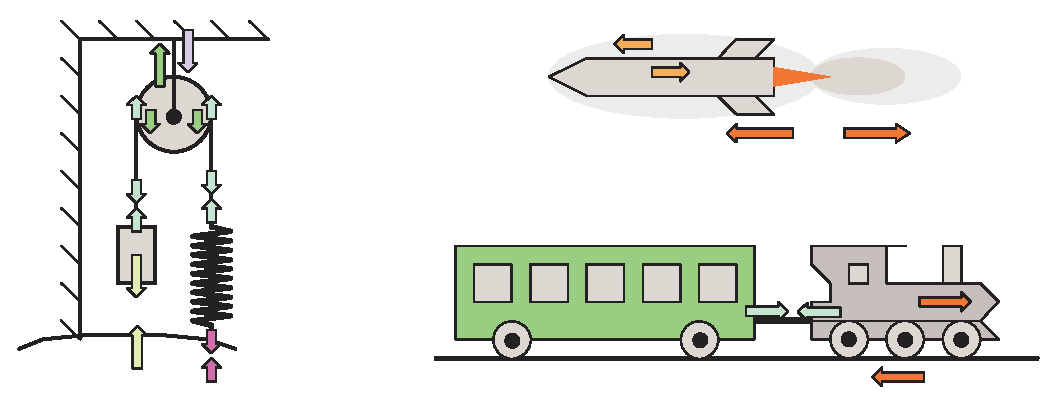
\includegraphics{GP003F05.eps}}
  \end{picture}\\[1mm]

Итак, если взаимодействуют 2 тела A и B ;) с массами $m_1$ и $m_2$, то оба приобретают противоположные ускорения:
\begin{displaymath}
\vec{a_1}=\frac{f_1}{m_1},\;\;\;\;\;\;\vec{a_2}=\frac{f_2}{m_2}
\end{displaymath}

Из 3зН следует, что $\vec{f_1}=-\vec{f_2}$, и поэтому
\begin{displaymath}
\vec{a_1}=-\frac{m_2}{m_1}\cdot\vec{a_2}
\end{displaymath}

Изменение количества движения тел A и B:
\begin{displaymath}
\vec{\Delta p_1}=\vec{f_1}\cdot\Delta t\;\;\;\;\;\;\;\vec{\Delta p_2}=
\vec{f_2}\cdot\Delta t=-\vec{\Delta p_1}
\end{displaymath}

\begin{center}
\fbox{\parbox{180mm}{\color{blue}\bf Насколько в результате взаимодействия импульс одного тела увеличился, настолько импульс другого тела уменьшился.}}\\[1mm]
\end{center}

Обобщая на всю систему из N тел, получаем ЗАКОН СОХРАНЕ\-НИЯ КОЛИЧЕСТВА ДВИЖЕНИЯ (ИМПУЛЬСА): $\sum\vec{p} = $const.

\begin{center}
\fbox{\parbox{180mm}{\color{blue}\bf Полный импульс замкнутой системы остается постоянным во все время движения. \color{red}\sl (Не обнаружено нарушений ни в микро-, ни в макро-мире, ни в квантовой, ни в релятивистской механике)}}
\end{center}

\newpage
Поскольку импульс --- это вектор, то закон сохранения выполняется отдельно для каждой его составляющей:

 \setlength{\unitlength}{1mm}
  \begin{picture}(180,50)(0,0)
   %\put(0,0){\framebox(180,65)[b]{}}
   \put(0,0){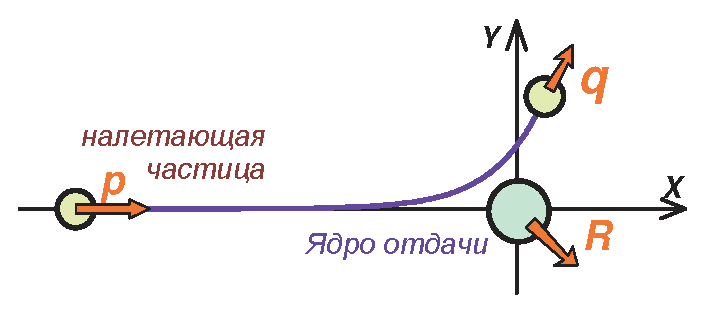
\includegraphics{GP003F06.eps}}
   \put(180,40){\makebox(0,0)[rt]{\parbox{60mm}{\begin{displaymath}
                                            \left\{ \begin{array}{ccc}
                                            p_x&=&R_x+q_x\\
                                            0&=&R_y+q_y\\
                                            0&=&R_z+q_z
                                                    \end{array}
                                            \right.
                                               \end{displaymath}}}}
  \end{picture}\\[1mm]

Для изолированной системы из N тел:

\begin{displaymath}
 \vec{P}=\sum_i^N\vec{p_i}=const\;\;\;\Leftrightarrow\;\;\;
 \left\{ \begin{array}{ccccc}
 P_x&=& \sum_{i=1}^N p_{xi}&=&const\\
 P_y&=& \sum_{i=1}^N p_{yi}&=&const\\
 P_z&=& \sum_{i=1}^N p_{zi}&=&const
 \end{array}
 \right.
\end{displaymath}
\hspace{3mm}

\underline{\bf Силы при криволинейном движении}

 \setlength{\unitlength}{1mm}
  \begin{picture}(180,80)(0,0)
   %\put(0,0){\framebox(180,90)[b]{}}
   \put(0,0){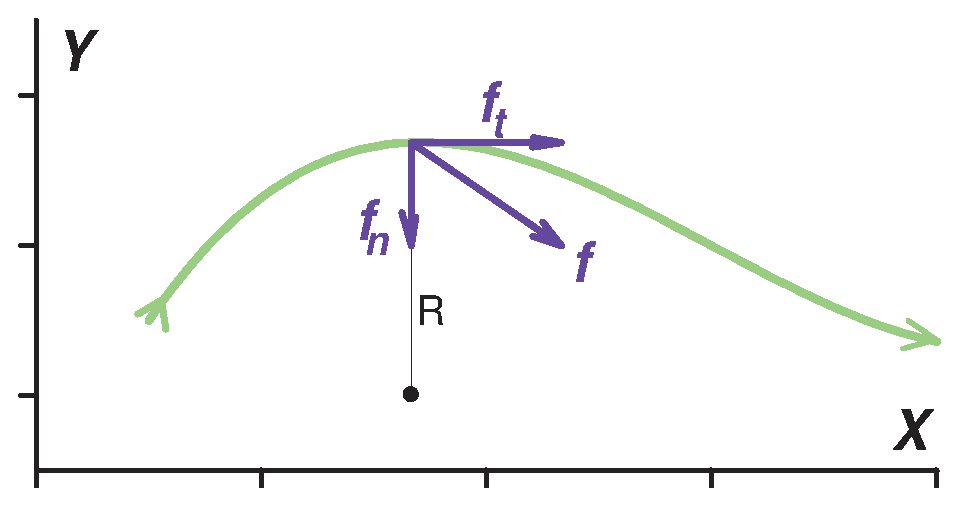
\includegraphics{GP003F07.eps}}
  \end{picture}\\

Как и ускорение, сила имеет 2 компонента: \begin{enumerate}
\item тенгенциальная сила ($\vec{f_t}\parallel\vec{v}$ -- разгоняет или тормозит)
\item центростремительная сила ($\vec{f_n}\perp\vec{v}$ -- заставляет менять направление)
\end{enumerate}
\begin{displaymath}
 \vec{f}=\vec{f_t}+\vec{F_n};\;\;\;\;\;\;\;|f|=\sqrt{f_t^2+f_n^2};\;\;\;\;\;\;\;\;
 |f_n|=ma_n=m \frac{v^2}{R}
\end{displaymath}

\newpage
\noindent
Равномерное движение по кривой: $f_t=0$. Вся сила -- центростремительная.\\[4mm]
Равномерное движение по окружности: $R=$const., $v=\omega R$
\begin{displaymath}
 f_n=m \frac{v^2}{R}=m\omega^2R=4\pi^2m\frac{R}{T^2}
\end{displaymath}

\underline{Центростремительная} сила приложена к телу, а равная ей (но противопо\-ложная по направлению) \underline{центробежная} -- к связям
\\
 \setlength{\unitlength}{1mm}
  \begin{picture}(180,60)(0,0)
   %\put(0,0){\framebox(180,65)[b]{}}
   \put(85,0){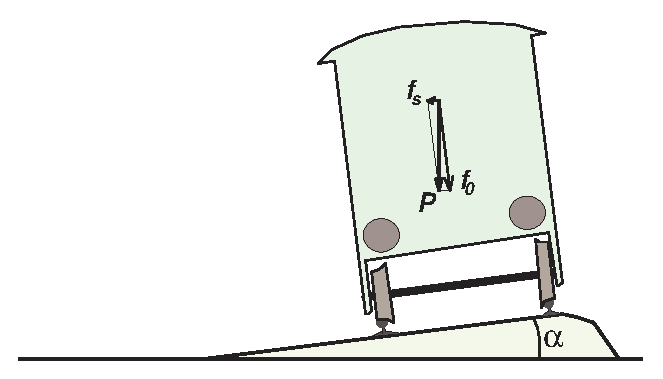
\includegraphics{GP003F08.eps}}
   \put(0,0){\makebox(0,0)[bl]{\parbox{130mm}{
    Неподвижный вагон, кроме нормальной к рельсам силы $f_0$, оказывает на них боковое давление с силой $f_s=P\;{\rm tg}\alpha$. Надо, чтобы при движении центробежная сила ее скомпенсировала:
   \begin{displaymath}
   P\cdot tg\alpha = mg\cdot tg\alpha = \frac{mv^2}{R}\;\;\;\;\Rightarrow\;\;\;
   tg\alpha = \frac{mv^2}{Rg}
   \end{displaymath}}}}
  \end{picture}\\[1mm]

\underline{\bf Ускоренные системы}
\\
 \setlength{\unitlength}{1mm}
  \begin{picture}(180,40)(0,0)
   %\put(0,0){\framebox(180,65)[b]{}}
   \put(0,0){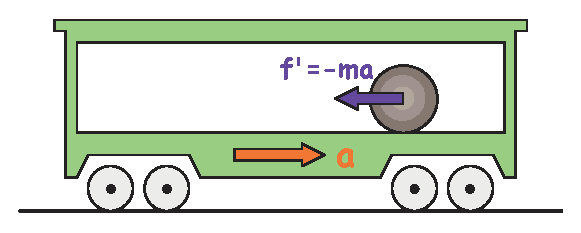
\includegraphics{GP003F09.eps}}
   \put(190,0){\makebox(0,0)[br]{\parbox{90mm}{
   В Лаб.системе: вагон ускоряется, шар отстает.\\
   В системе вагона: шар покатился назад с ускорением $-a$, как если бы появилась сила
   $\vec{f}=-m\vec{a}$
   }}}
  \end{picture}\\[1mm]

Фиктивная сила, которую приходится вводить в ускоренной системе отсчета, чтобы в ней выполнялся 2 закон Ньютона -- \underline{инерционная сила} или \underline{сила инерции}.
\\
 \setlength{\unitlength}{1mm}
  \begin{picture}(180,90)(0,0)
   %\put(0,0){\framebox(180,80)[b]{}}
   \put(0,0){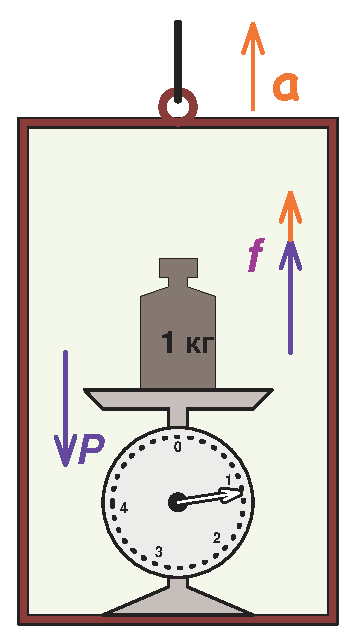
\includegraphics{GP003F10.eps}}
   \put(190,0){\makebox(0,0)[br]{\parbox{130mm}{
   \begin{enumerate}
   \item{\bf $\vec{a}=0$ (Лифт стоит на месте или движется равномерно.)}
        Гиря давит на весы своим весом $\vec{P}=m\vec{g}$. Весы давят на гирю с такой же силой и уравновешивают ее вес. (В обеих {\bf инерциальных} системах координат)
   \item{\bf $\vec{a}>0$ (Лифт ускоряется вверх.)}
    \begin{itemize}
    \item В Лаб.системе: Чтобы гиря тоже начала ускоряться вместе с лифтом, весы давят на нее снизу с дополнительной силой $\vec{f\prime}=m\vec{a}$. По 3зН гиря давит на весы с такой же силой.
    \item В системе лифта: появилась сила инерции $\vec{f\prime\prime}=-m\vec{a}$, которая добавилась к весу гири.
    \end{itemize}
   \end{enumerate}
   }}}
  \end{picture}\\[1mm]
  ОТО Эйнштейна: Вселенная относительно системы лифта дернулась вниз с ускорением $-\vec{a}$ и создала дополнительное гравитационное поле, направ\-ленное туда же:
   $g\;\;\;\rightarrow\;\;\;g\prime=(g+a)$.\\[1mm]

\underline{\bf Вращающиеся системы}
\\
 \setlength{\unitlength}{1mm}
  \begin{picture}(180,100)(0,0)
   %\put(0,0){\framebox(180,65)[b]{}}
   \put(0,0){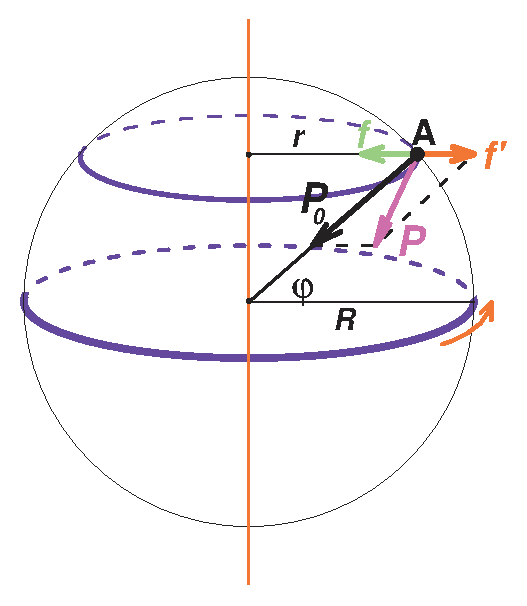
\includegraphics{GP003F11.eps}}
   \put(190,0){\makebox(0,0)[br]{\parbox{100mm}{
   В инерциальной гелиоцентрической системе: чтобы тело А на широте $\varphi$ вращалось вместе с Землей вокруг ее оси, надо, чтобы часть его веса $P_0$ играла роль центростремительной силы ${\color{green}f}=m\omega^2r=m\omega^2R\cos\varphi$.\\
   В системе, связанной с Землей: 1) направленный к центру Земли вес $P_0$  и 2) {\sl инерционная центробежная сила} ${\color{red}f\prime}=m\omega^2r$, направленная от оси. Их сумма - кажущийся вес ${\color{magenta}P}$.\\
   Масштаб: $f/P_0=\omega^2R\cos\varphi/g\simeq\cos\varphi/289$
   }}}
  \end{picture}\\[1mm]
На экваторе ($\varphi=0$): $f/P_0$ -- максимально; \hfill{} $f_{\max}/P_0=\omega^2R/g=v^2/gR$\\
Обращается в 1 при $v=\sqrt{gR}\simeq7.9$ км/с
\newpage
\centerline{\underline{\bf Сила Кориолиса}}
 \setlength{\unitlength}{1mm}
  \begin{picture}(180,240)(0,0)
   %\put(-5,-10){\framebox(180,240)[b]{}}
   \put(0,-10){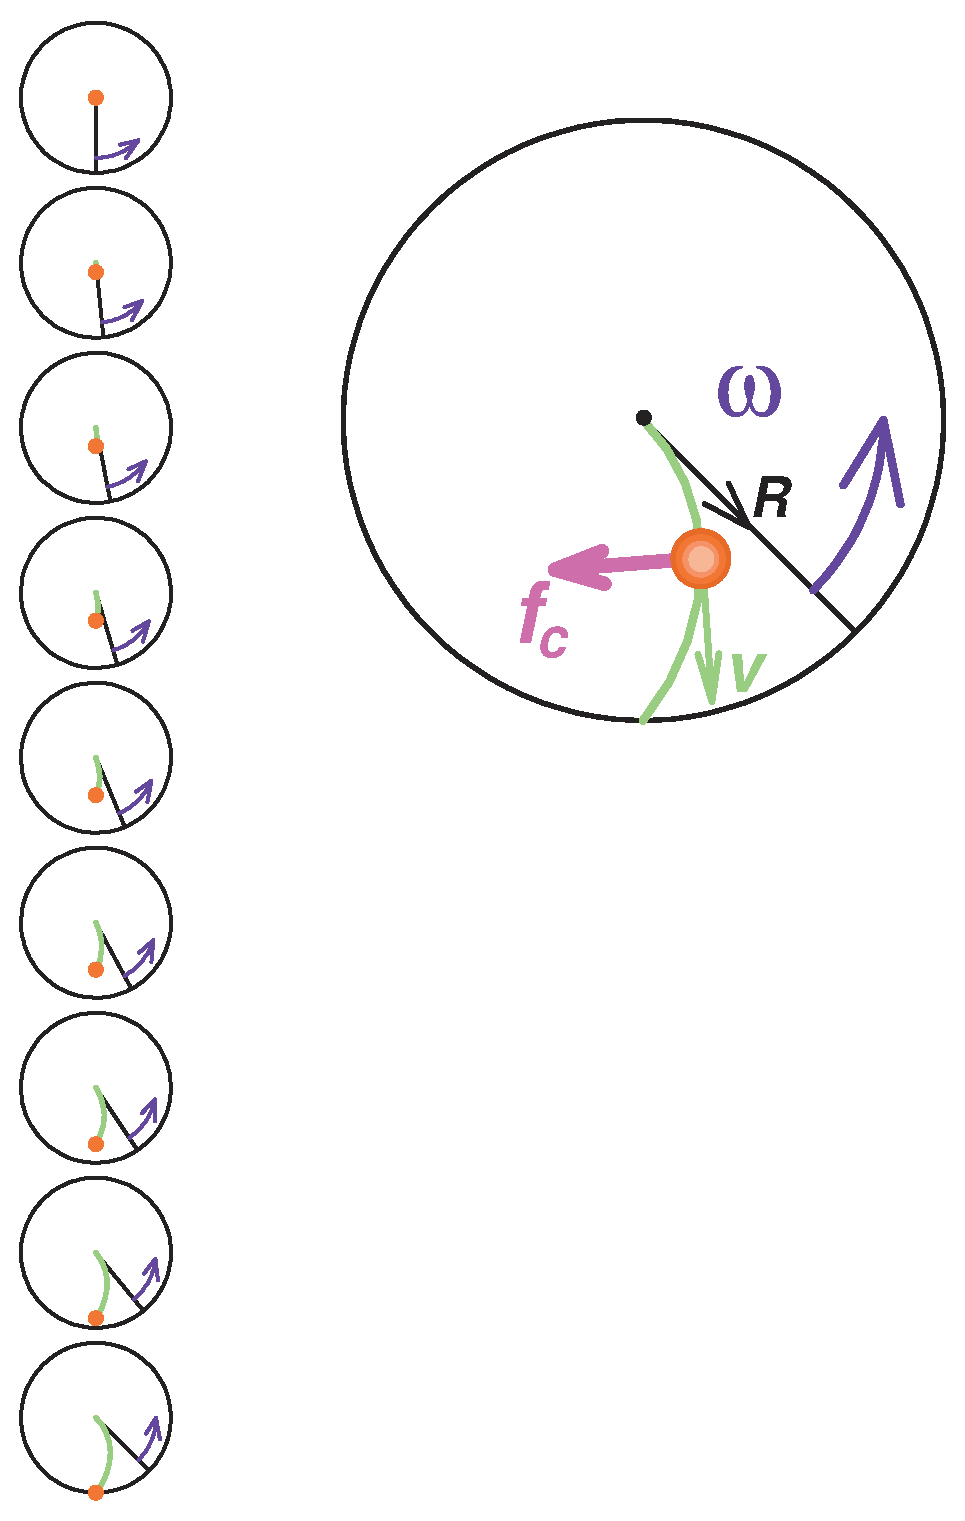
\includegraphics{GP003F12.eps}}
   \put(100,231){\makebox(0,0)[c]{Шарик катится по вращающемуся диску:}}
   \put(35,120){\makebox(0,0)[tl]{\parbox{40mm}{В лабораторной (инерциальной!) системе -- O.K. }}}
   \put(180,115){\makebox(0,0)[tr]{\parbox{80mm}{В системе диска шарик сносит вправо, как если бы на него действовала сила $\vec{f_c}\perp\vec{v}$}}}
   \put(180,0){\makebox(0,0)[br]{\parbox{150mm}{Мы живем в такой вращающейся системе. Чтобы корректно объяснить все явления, у нас $\exists$ два выхода:
   \begin{enumerate}
   \item Каждый раз переделывать все формулы, учитывая вращение системы координат
   \item Ввести фиктивную (как и силу инерции) Кориолисову силу $\vec{f_c}$, которая $\perp$ скорости $\vec{v}$ и оси вращения $\vec{\omega}$.
   \end{enumerate}
   \begin{displaymath}
    \vec{f_c}=2m\left[\vec{v}\times\vec{\omega}\right]
   \end{displaymath}
   }}}
  \end{picture}\\[1mm]
\underline{\bf Вывод формулы для силы Кориолиса} \hfill{ } {\color{green}\sl (факультативно)}

Пусть тело движется со скоростью $\vec{v}$ и ускорением $\vec{a}$ в неинерциальной системе координат, которая вращается с угловой скоростью $\vec{\omega}$ и угловым ускорением $\vec{\beta}$. Если радиус вращения тела равен $\vec{R}$,
то линейная скорость $\vec{v\prime}$ во внешней \underline{инерциальной} системе равна:
   \begin{displaymath}
    \vec{v\prime}= \vec{v}+\left[\vec{\omega}\times\vec{R}\right]
   \end{displaymath}
 Ускорение $\vec{a\prime}$ этой инерциальной системе равно:
   \begin{displaymath}
   \vec{a\prime}= \frac{d}{dt}\left(\vec{v\prime}\right) =
   \frac{d}{dt}\left(\vec{v}\right) +
   \frac{d}{dt}\left[\vec{\omega}\times\vec{R}\right]=
   \frac{d}{dt}\left(\vec{v}\right) +
   \left[\frac{d}{dt}\left(\vec{\omega}\right)\times\vec{R}\right] +
   \left[\vec{\omega}\times\frac{d}{dt}\left(\vec{R}\right)\right]\;.
   \end{displaymath}
 Учитывая, что
   \begin{displaymath}
   \frac{d}{dt}\left(\vec{v}\right) = \vec{a}+\left[\vec{\omega}\times\vec{v}\right],
   \end{displaymath}
 а скорость изменения радиуса
   \begin{displaymath}
   \frac{d}{dt}\left(\vec{R}\right) = \vec{v}+\left[\vec{\omega}\times\vec{R}\right],
   \end{displaymath}
получим:
   \begin{displaymath}
   \vec{a\prime}=
   \vec{a}+
   \left[\vec{\omega}\times\vec{v}\right]+
   \left[\vec{\beta}\times\vec{R}\right]+
   \left[\vec{\omega}\times\vec{v}\right]+
   \left[\vec{\omega}\times\left[\vec{\omega}\times\vec{R}\right]\right].
      \end{displaymath}
Далее воспользуемся свойством тройного векторного произведения
   \begin{displaymath}
\left[\vec{A}\times\vec{B}\times\vec{C}\right] =
\vec{B}\cdot\left(\vec{A}\cdot\vec{C}\right) -
\vec{C}\cdot\left(\vec{A}\cdot\vec{B}\right),
      \end{displaymath}
а также тем фактом, что векторы $\vec{\omega}$ и $\vec{R}$ взаимно перпендикулярны, и потому их скалярное произведение равно нулю:
   \begin{displaymath}
   \left[\vec{\omega}\times\left[\vec{\omega}\times\vec{R}\right]\right]=
   \vec{\omega}\cdot\left(\vec{\omega}\cdot\vec{R}\right)-
   \vec{R}\cdot\left(\vec{\omega}\cdot\vec{\omega}\right)=
   -\vec{R}\cdot\omega^2.
   \end{displaymath}
Итак, получаем, что ускорение тела относительно инерциальной системы, в которой просто обязаны соблюдаться все законы Ньютона, равно:
   \begin{displaymath}
   \vec{a\prime}=
   \vec{a}+
   \left[\vec{\beta}\times\vec{R}\right]-
   2\left[\vec{v}\times\vec{\omega}\right]-
   \omega^2\vec{R}.
   \end{displaymath}
 Если почленно умножить все это на массу $m$, то в последнем слагаемом узнаем центростремительную силу, которая должна уравновесить силу инерции, направленную по радиусу, а в предпоследнем - силу, которая должна скомпенсировать силу Кориолиса (если мы не хотим, чтобы тело отклонилось от своего заданного движения в неинерциальной системе).

\end{document} 